\chapter{Electrical Design}
\section{Introduction}
The electronics of the robot use a combination of off-the-shelf parts and custom designed circuits. A microcontroller handles low-level hardware control and interfacing such as reading sensors and supplying motor driver control signals while a Raspberry Pi microcontroller processes the data within the artificial neural network and determines motor speeds and directions. The two processors communicate through a 921,600 baud UART link. During development, the robot used either a 2015 MacBook Pro or desktop computer instead of the Raspberry Pi to simplify programming and omit limitations imposed by the Pi's lower processing speed.

\section{Power}
A four cell, 1800 mAH lithium polymer (LiPo) battery powers the entire system. The battery is connected using polarized XT60 connectors to prevent reverse connection. The battery voltage varies between 16.8 V when fully charged and 14.8 V when depleted so two off-the-shelf DC-DC switching regulators, shown in Figure \ref{fig:smps}, buck battery voltage down to 12 V and 7 V supplies. The switching regulators accept a 7 -- 40 V supply and can output 1.2 -- 35 V at 8 A each. The 12 V bus powers the three motor drivers boards while the 7 V bus powers the STM32 Nucleo-64 development board and two AZ1085CD low-dropout linear regulators (LDO). One LDO produces a 5 V bus while the other provides 3.3 V, each at 3 A. 

\begin{figure}[H]   % [h] means here
	\centering 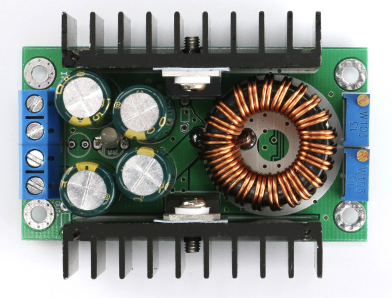
\includegraphics[width=6in, height=3.85in, keepaspectratio]{figures/smps.png}
	\caption{DC-DC Buck Regulator \cite{smps}}\label{fig:smps}
\end{figure}

\section{Sensors}
The robot uses five off-the-shelf sensors for determining its position: four VL53L0X 1-D LIDAR rangefinders and one Adafruit 9-DOF inertial measurement unit (IMU).

\subsection{Adafruit 9-DOF IMU}
The Adafruit 9-DOF IMU incorporates the L3DG20H gyroscope and LSM303DLHC accelerometer/compass combo on a single carrier board to allow full inertial measurement in a convenient form factor \cite{adafruit_imu}. Figure \ref{fig:imu} shows the IMU mounted in the 3D printed bracket. The robot only utilizes the accelerometer and magnetic compass to realize a tilt-compensated compass. The LSM303DLHC can measure both acceleration and magnetic fields in three dimensions with configurable bandwidth and full-scale ranges. It uses 400 kHz I\textsuperscript{2}C for control and data transfer and draws power from the 3.3 V supply. Raw measurements from the IMU possess significant offset and scaling error so a calibration routine is required.

\begin{figure}[H]   % [h] means here
	\centering 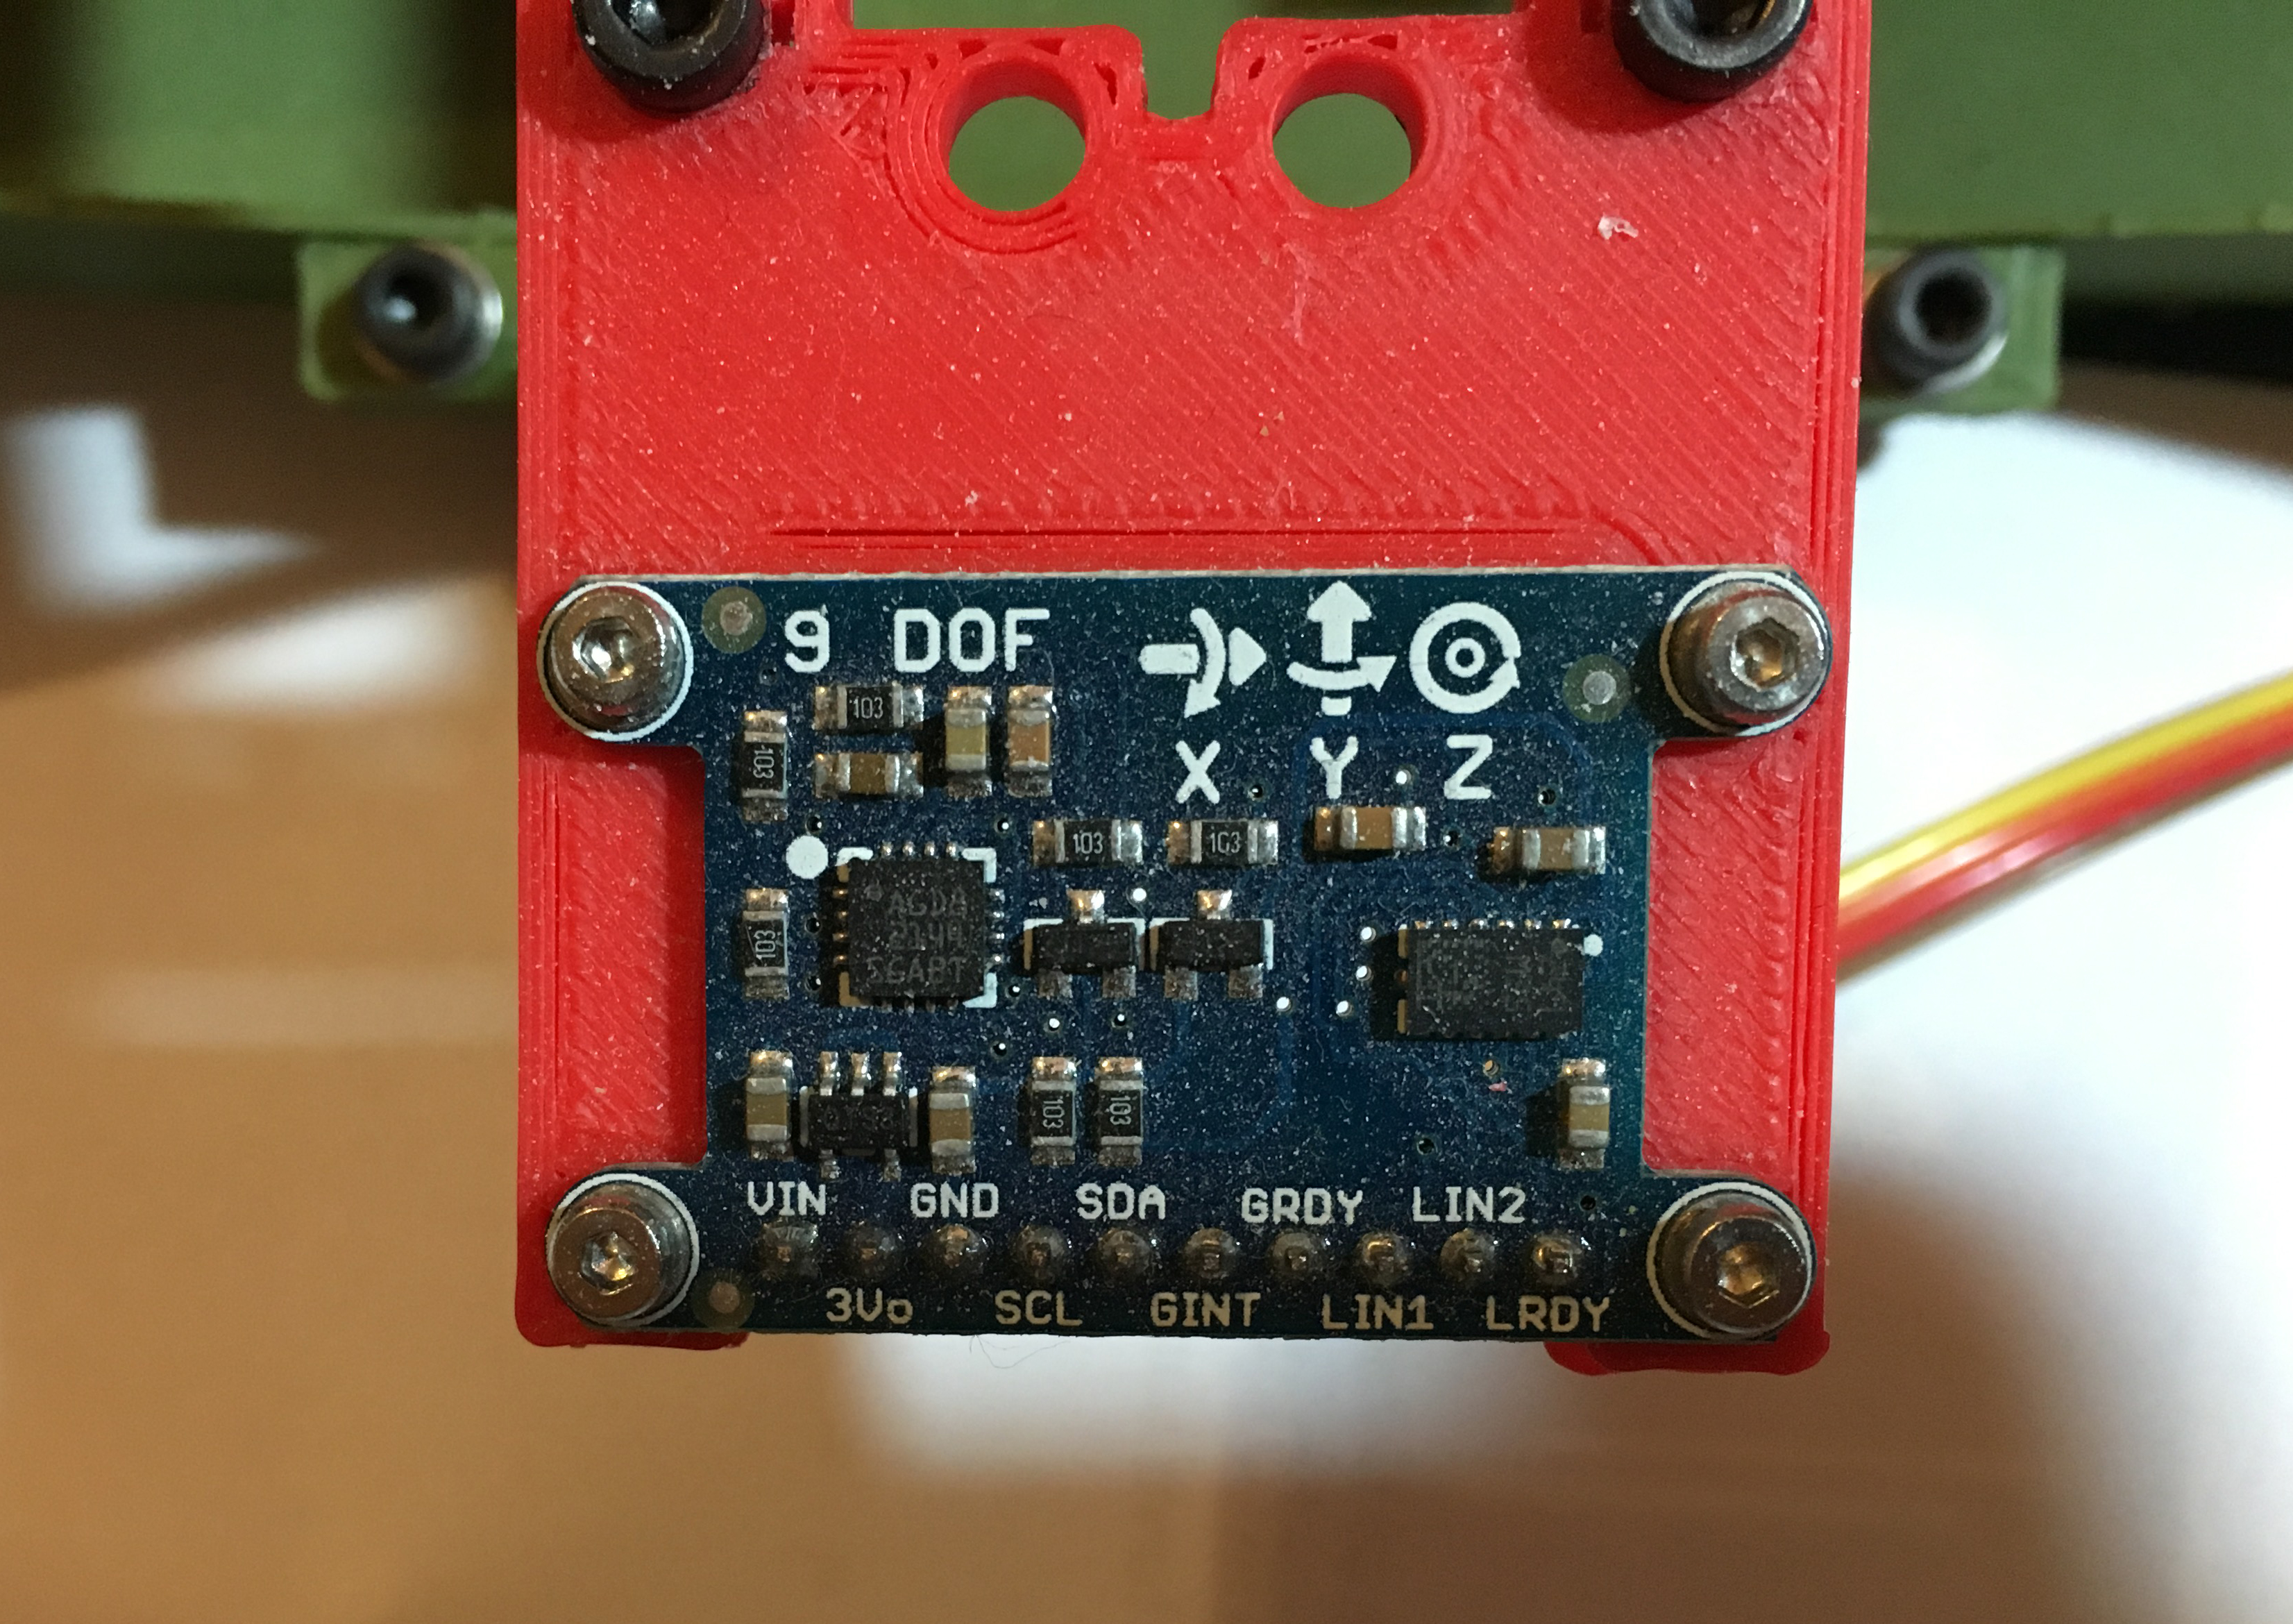
\includegraphics[width=6in, height=3.85in, keepaspectratio]{figures/imu.png}
	\caption{Adafruit 9-DOF IMU Mounted}\label{fig:imu}
\end{figure}

The accelerometer and magnetometer calibration process utilizes the FreeIMU program written by Fabio Varesano in Python \cite{freeimu}. The program features a graphical user interface (GUI), shown in Figure \ref{fig:cal_gui},  to display accelerometer and magnetometer measurements in real time and plots them in 3D space. The calibration program was originally designed to calibrate the open-source FreeIMU IMU when connected to an Arduino with the FreeIMU calibration firmware so the program's device communication back-end was modified to accept the LSM303DLHC IMU connected to an STM32 microcontroller with custom firmware. The calibration algorithm assumes that the sensor's measurements are linearly distorted and therefore produces a linear scaling factor and offset for each of six measurements (accelerometer X, Y, Z and magnetometer X, Y, Z). The correction algorithm is shown below where $val$ can represent any of the six measurements.

\begin{equation}
val_{calibrated} = m_{scale} val_{measurement} + b_{offset}
\end{equation}

\begin{figure}[H]   % [h] means here
	\centering 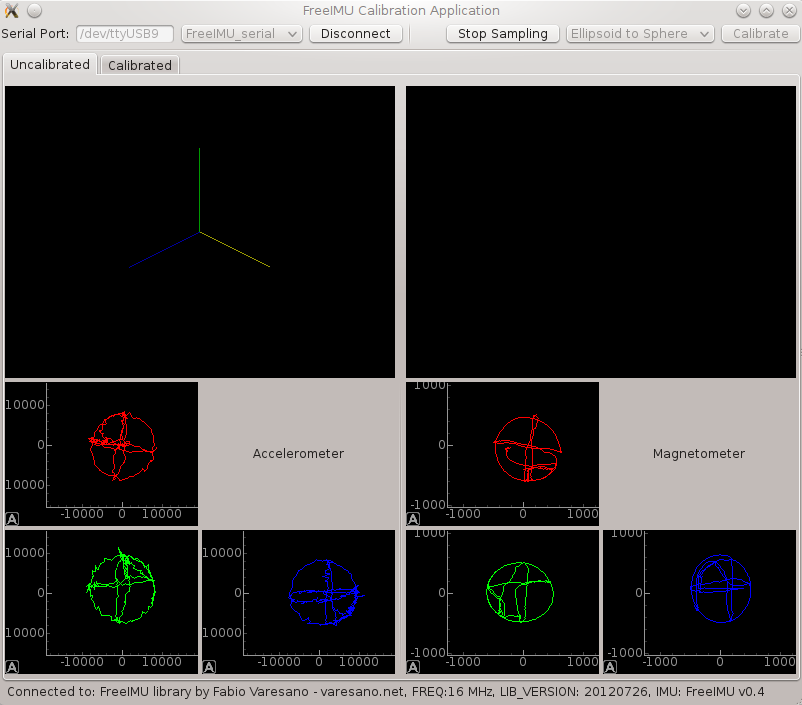
\includegraphics[width=6in, keepaspectratio]{figures/cal_gui.png}
	\caption{FreeIMU GUI \cite{freeimu}}\label{fig:cal_gui}
\end{figure}

The calibration procedure is as follows:
\begin{enumerate}
	\item \ssp IMU should be mounted on fully assembled robot and connected to microcontroller.
	\item \ssp Connect microcontroller serial port to computer through Serial-to-USB converter.
	\item \ssp Click "Begin Sampling" to start recording magnetometer and accelerometer measurements.
	\item \ssp Point the IMU x-axis at the ground and rotate \ang{360} around that axis. Repeat for y-axis and z-axis.
	\item \ssp Point the IMU x-axis at the sky and rotate \ang{360} around that axis. Repeat for y-axis and z-axis.
	\item \ssp Repeat Steps 3 and 4 at least twice to increase data size.
	\item \ssp Click "Stop Sampling".
	\item \ssp Click "Calibrate" to calculate scaling and offset constants.
\end{enumerate}

The procedure ensures that ends of each axis eventually receive the maximum acceleration and magnetic field. To ensure hard-iron errors (such as from motors and permanent magnets) as well as soft iron errors (from local ferromagnetic materials like steel) are compensated for in the calibration, the process should be performed with the fully assembled robot and redone each time the robot is modified \cite{hard_soft_correction}. Since the expected fields are known (acceleration due to gravity, strength of Earth's magnetic field), the required linear transformation can be calculated. See \cite{freeimu} for details of the exact algorithm.

\subsection{VL53L0X Rangefinders}
The rangefinders, marketed by STMicroelectronics as the "world's smallest Time-of-Flight ranging sensor", are capable of measuring between 30 and 2000 mm with a 30 Hz sample rate \cite{vl53l0x}. It operates by firing pulsed light from a vertical cavity surface emitting laser (VCSEL), measuring time taken for the laser pulse to reflect back to the sensor, and calculating the distance based on the known speed of light. The robot uses cheap \$8 VL53L0X breakout boards in lieu of designing and assembling custom carriers; the sensor itself comes in a 4.4 x 2.4 mm lead-less package making hand soldering prohibitively difficult. Figure \ref{fig:rangefinder} shows the sensor board mounted in the 3D printed bracket. The sensor breakout boards include the VL53L0X module, decoupling capacitors, an LDO for the sensor's 2.8 V power supply, and level shifters for the I\textsuperscript{2}C lines. Control and data transfer both occur over 400 kHz I\textsuperscript{2}C so the breakout only requires four wires: 3.3 V, ground, and the I\textsuperscript{2}C data and clock lines. To characterize the accuracy and precision of the sensor, distance measurements were taken by targeting the sensor at a sheet of standard white printer paper. The data is compared with measurements from a tape measure; results are shown in Figure \ref{fig:rangefinder_measurement}. 

\begin{figure}[H]   % [h] means here
	\centering 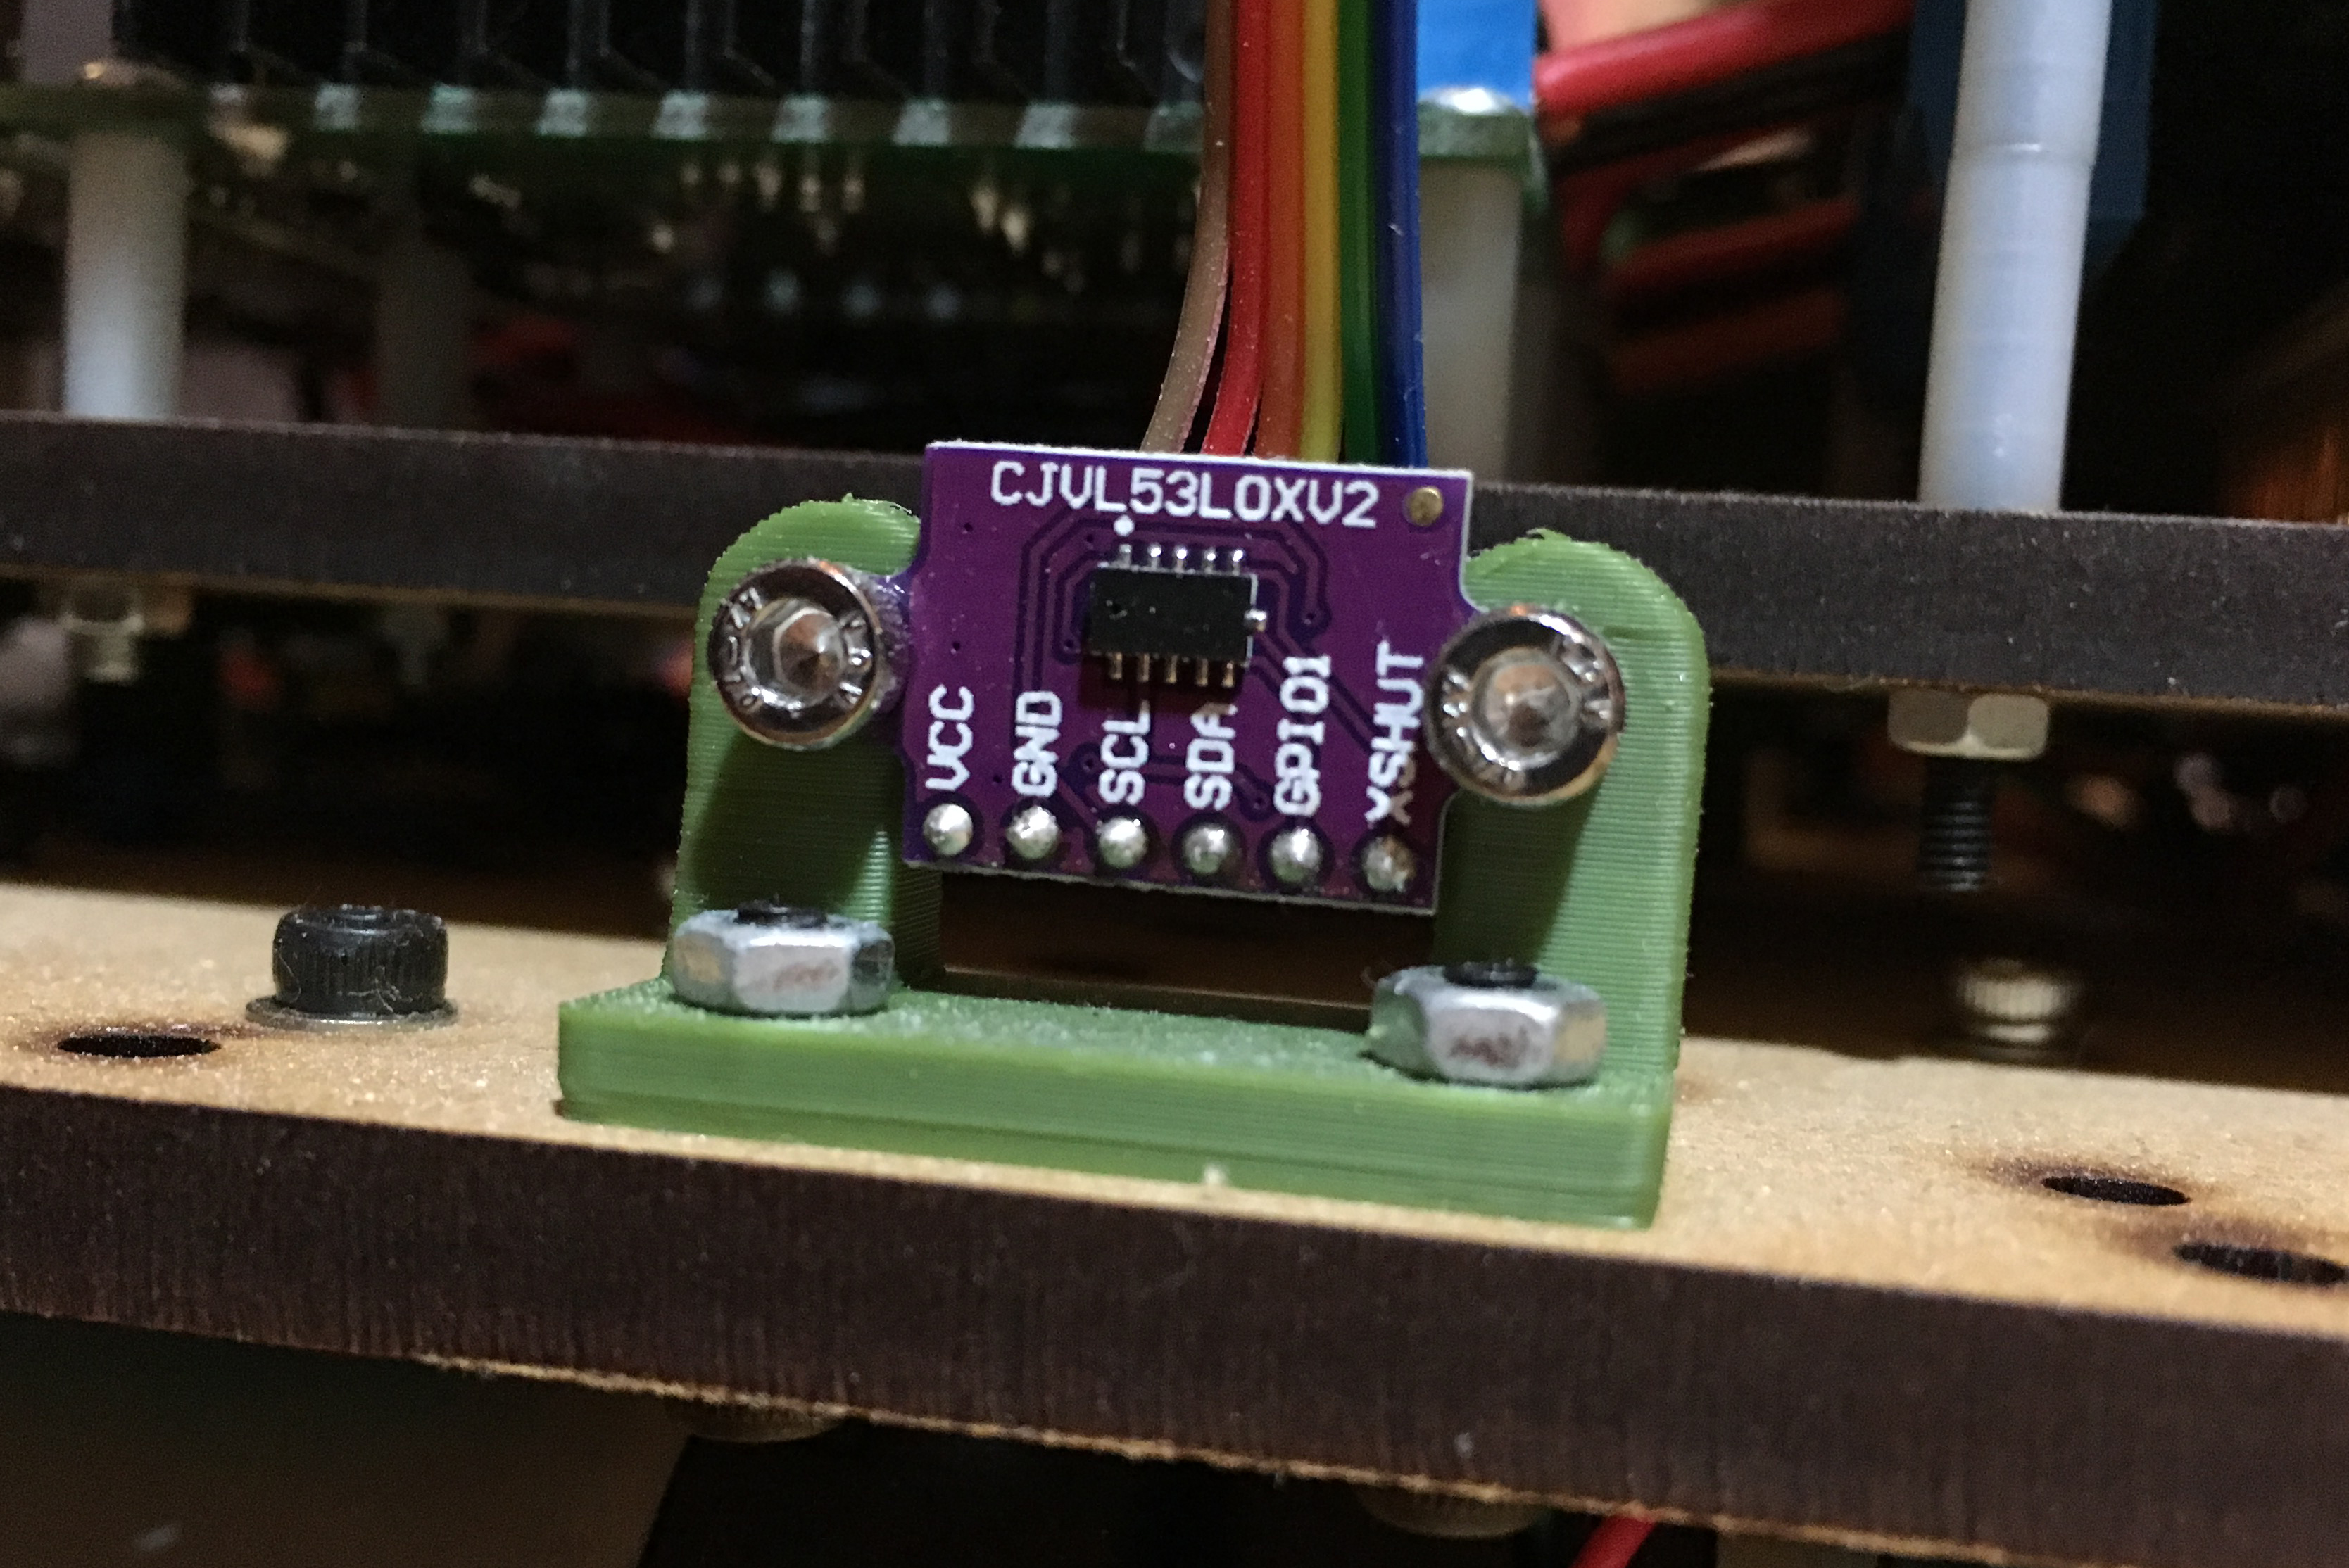
\includegraphics[width=6in, height=3.85in, keepaspectratio]{figures/rangefinder.png}
	\caption{VL53L0X Rangefinder Mounted}\label{fig:rangefinder}
\end{figure}

\begin{figure}[H]   % [h] means here
	\centering 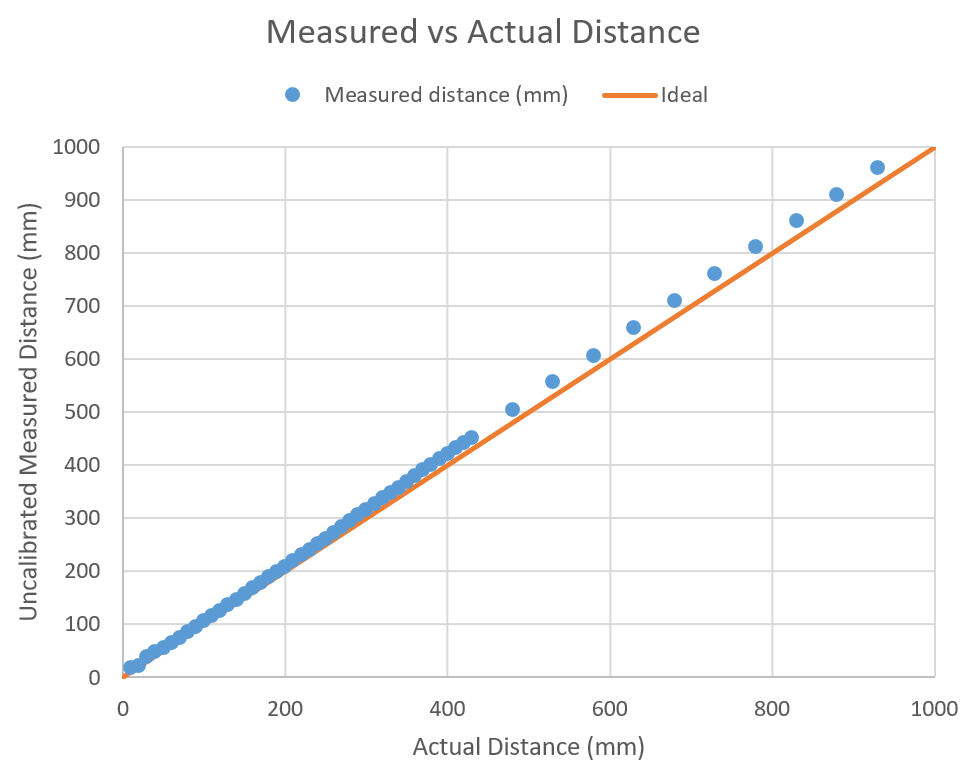
\includegraphics[width=6in, height=3.85in, keepaspectratio]{figures/rangefinder_measurement.png}
	\caption{VL53L0X Measured vs. Actual Distance}\label{fig:rangefinder_measurement}
\end{figure}

Since the measurements are linear, only a linear correction is required as follows:
\begin{equation}
	d_{calibrated} = m_{scale} d_{measurement} + b_{offset}
\end{equation}
where $d_{measurement} $ is distance as returned by the sensor, $m_{scale} = 0.96502507$, $b_{offset} = -3.8534743$, and $d_{calibrated}$ is the calibrated distance. The squared error for each data point before and after calibration is shown in Figure \ref{fig:rangefinder_calibrated}. The mean squared error for the uncalibrated data points is 342.3 mm and 15.0 mm after calibration, indicating the use of an appropriate model and constants.

\begin{figure}[H]   % [h] means here
	\centering 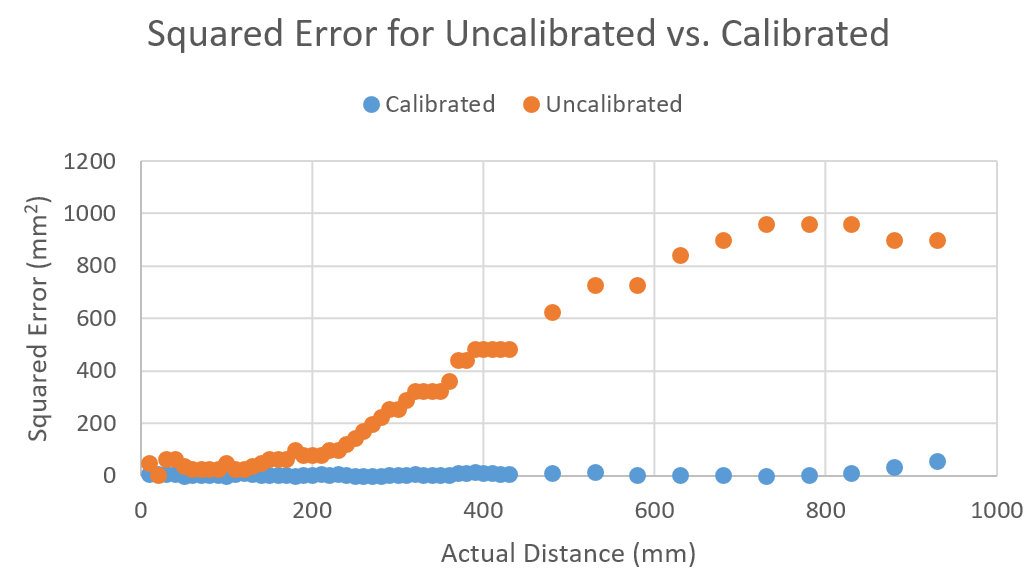
\includegraphics[width=6in, height=3.85in, keepaspectratio]{figures/rangefinder_calibrated.png}
	\caption{VL53L0X Squared Error for Uncalibrated vs. Calibrated}\label{fig:rangefinder_calibrated}
\end{figure}

Additionally, 100 measurements were taken at each distance and the variance computed to characterize the spread. The results are shown in \ref{fig:rangefinder_stddev}. The rangefinders are very accurate; at 900 mm with calibration, the error is only 7 mm or 0.8\% error. Of course, this error is with respect to the average measurement at 900 mm. At 900 mm, the standard deviation is 14 mm so individual measurements can vary, especially with non-ideal surfaces. The closer the target, the more accurate and less varied the measurement. No experiments were carried out to determine the measurement characteristics on various colored, textured, transparent, or angled surfaces as the expected target surface is white painted wood.

\begin{figure}[H]   % [h] means here
	\centering 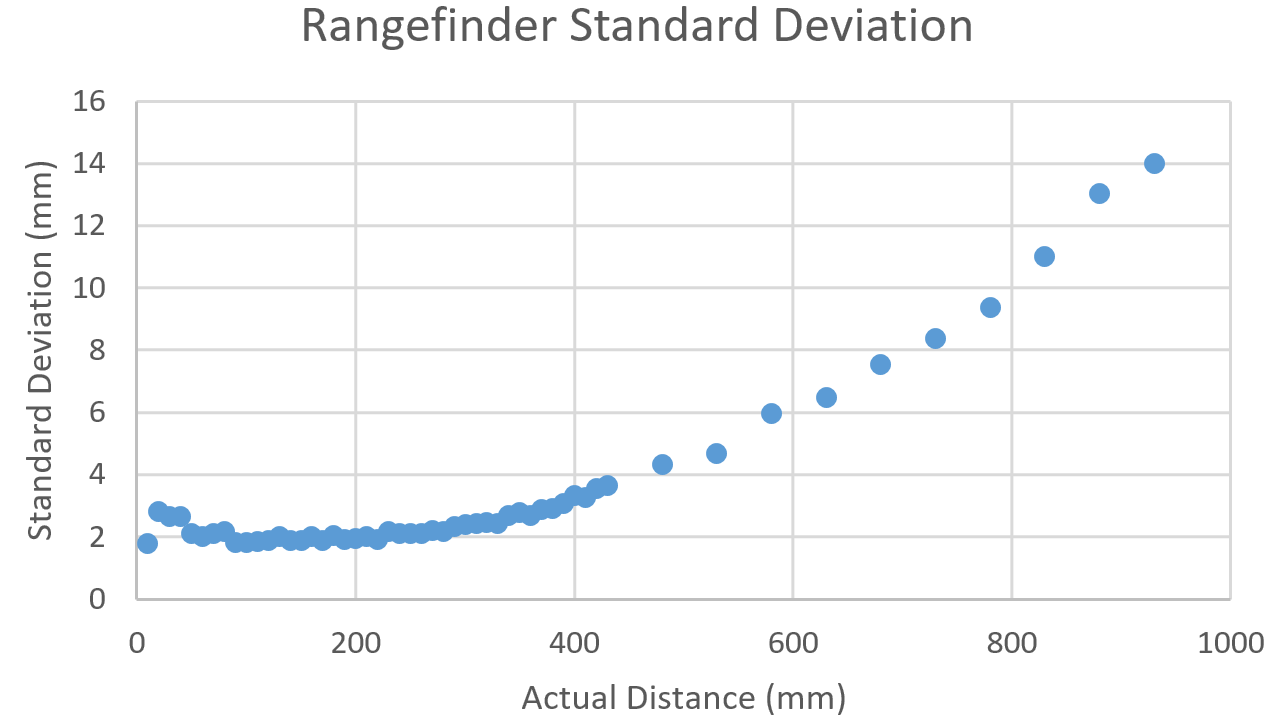
\includegraphics[width=6in, height=3.85in, keepaspectratio]{figures/rangefinder_stddev.png}
	\caption{VL53L0X Standard Deviation}\label{fig:rangefinder_stddev}
\end{figure}

\section{Motors}
The robot uses four 12V Pololu 37D motors to drive the wheels. The motors draw 630 mA each at full speed steady state of 234 rpm (24.46 rad/s) and have a maximum acceleration of 4,100 rpm/s (430 rad/s\textsuperscript{2}).

\section{Motor Drivers}
The system uses three off-the-shelf L298N motor driver boards since they are easily obtainable for less than \$6 each and incorporate features such as heat-sinking, flyback voltage protection, supply filtering, and screw terminal connections. Implementing comparable motor drivers with a similar feature set would undoubtedly cost more. Each L298N is a dual H-bridge driver with 2 A maximum output per bridge using a 5 -- 35 V supply. Two motor drivers handle the four robot drive motors while the third powers the blower fan and shooting mechanism motors. 

Figure \ref{fig:l298n} shows a wiring diagram for each motor driver. The board uses four digital control inputs, each controlling the state of one half-bridge. Each motor uses a pair of inputs: IN1 and IN2 control one motor while IN3 and IN4 control the other. To achieve direction and speed control, IN1 and IN3 are pulse width modulated (PWM) while IN2 and IN4 are digitally set. Table \ref{tab:L298N_truth_table} is a truth table of the motor state versus inputs.

\begin{figure}[H]   % [h] means here
	\centering 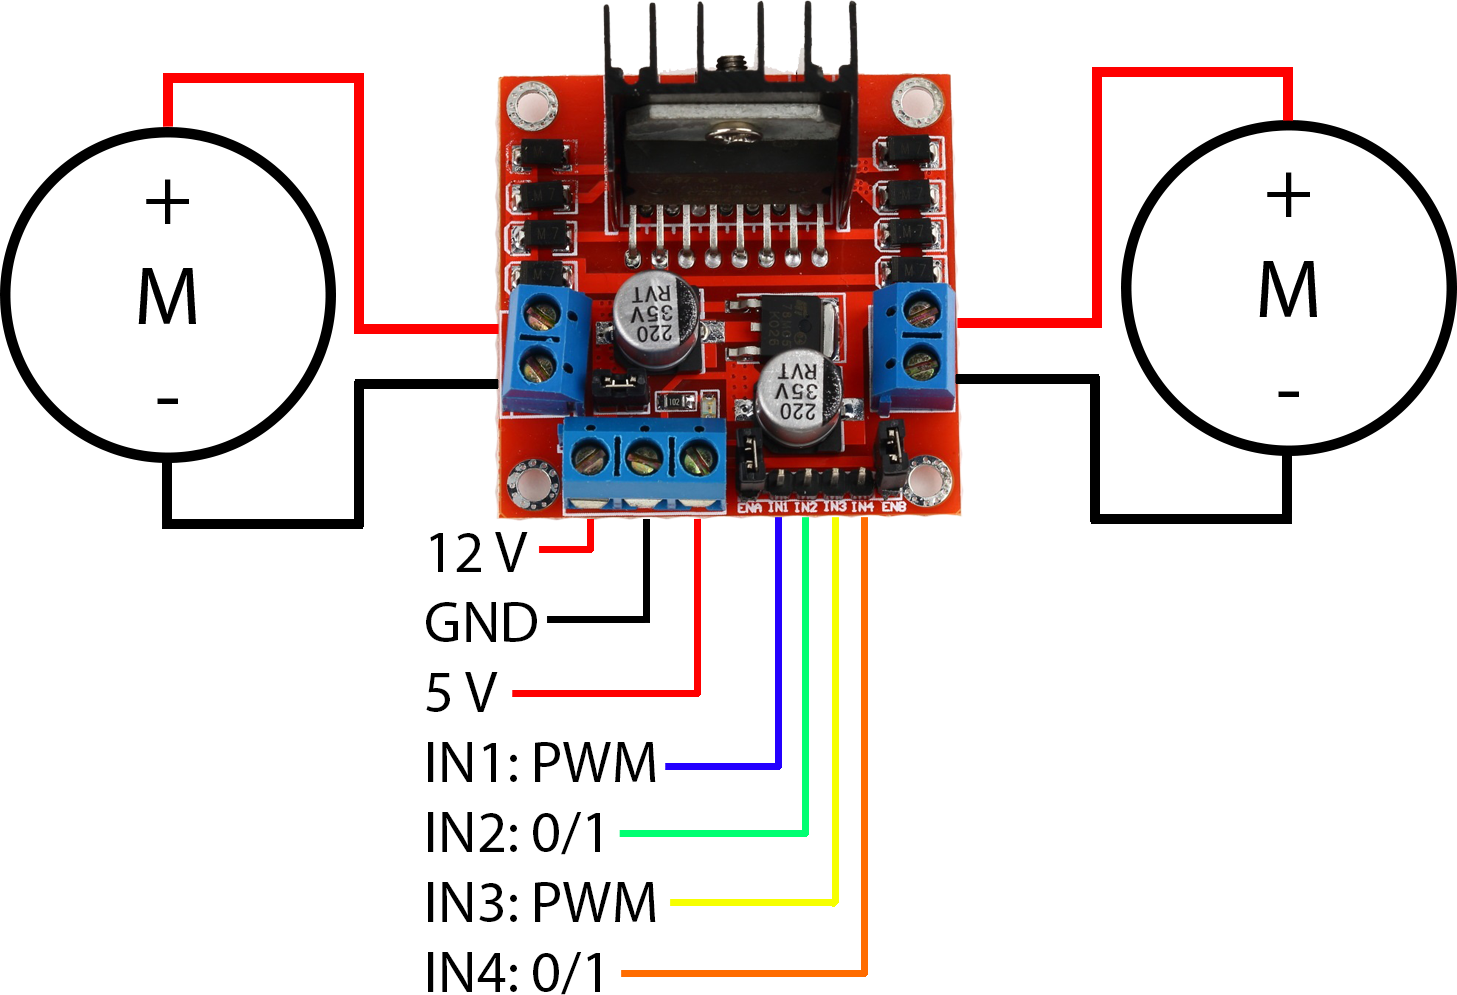
\includegraphics[width=6in, height=3.85in, keepaspectratio]{figures/l298n.png}
	\caption{L298N Motor Driver Wiring Diagram \cite{l298n}}\label{fig:l298n}
\end{figure}

\begin{table}[h]
	\centering	\caption{Motor Control Truth Table}
	\begin{tabular}{ccc}
		\hline 
		IN1/IN3 Duty Cycle & IN2/IN4 State & Motor State \\ 
		\hline 
		0\% & 0 & Stopped \\ 
		\hline 
		\textgreater 0\% & 0 & Forward, speed increases with duty cycle \\ 
		\hline 
		\textless 100\% & 1 & Reverse, speed decreases with duty cycle \\ 
		\hline 
		100\% & 1 & Stopped \\ 
		\hline 
	\end{tabular} 
	\label{tab:L298N_truth_table}
\end{table}

\section{Servo}
A GWS S03N standard servo powered from the 5 V bus actuates the gating mechanism in the ball hopper. Most servos are controlled by driving the control wire with a pulse width modulated (PWM) signal with a period of 15 -- 25 ms and a pulse width between 0.5 ms and 2.5 ms where the pulse width determines the position of the servo as shown in Figure \ref{fig:servo_pulse_width}. 

\begin{figure}[H]   % [h] means here
	\centering 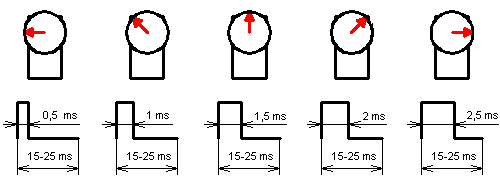
\includegraphics[width=6in, height=3.85in, keepaspectratio]{figures/servo_pulse_width.png}
	\caption{Servo PWM Control Scheme \cite{servo_pulse_width}}\label{fig:servo_pulse_width}
\end{figure}

Due to cheap manufacturing and loose tolerances, the actual required pulse widths can vary from servo to servo, requiring calibration to obtain accurate positional control. The process for calibration is simple: apply various pulse widths and record the resulting servo positions. The calibrated pulse widths and servo angles are recorded in Table \ref{tab:servo_angles}.

\begin{table}[h]
	\centering	\caption{Servo Required Pulse Widths}
	\begin{tabular}{cc}
		\hline 
		Servo Position & Pulse Width (ms) \\ \hline 
		\ang{0} & 0.674 \\ \hline 
		\ang{45} & 1.082 \\ \hline 
		\ang{90} & 1.490 \\ \hline 
		\ang{135} & 1.898 \\ \hline 
		\ang{180} & 2.306 \\ \hline 
	\end{tabular} 
	\label{tab:servo_angles}
\end{table}

\section{Microcontroller}
An STMicroelectronics STM32F446RE microcontroller (MCU) serves as the bridge between the robot's low-level electronics and the high-level control system running on a desktop computer. Specifically, the MCU collects data from sensors over I\textsuperscript{2}C and general purpose input/output (GPIO), generates control signals for the motor drivers and servo, and services commands from UART (universal asynchronous receiver-transmitter). The MCU resides on an STMicroelectronics Nucleo-64 development board, shown in Figure \ref{fig:nucleo64}, which conveniently integrates an ST-LINK V2 debugger, programmer, and USB-to-UART interface.

\begin{figure}[H]   % [h] means here
	\centering 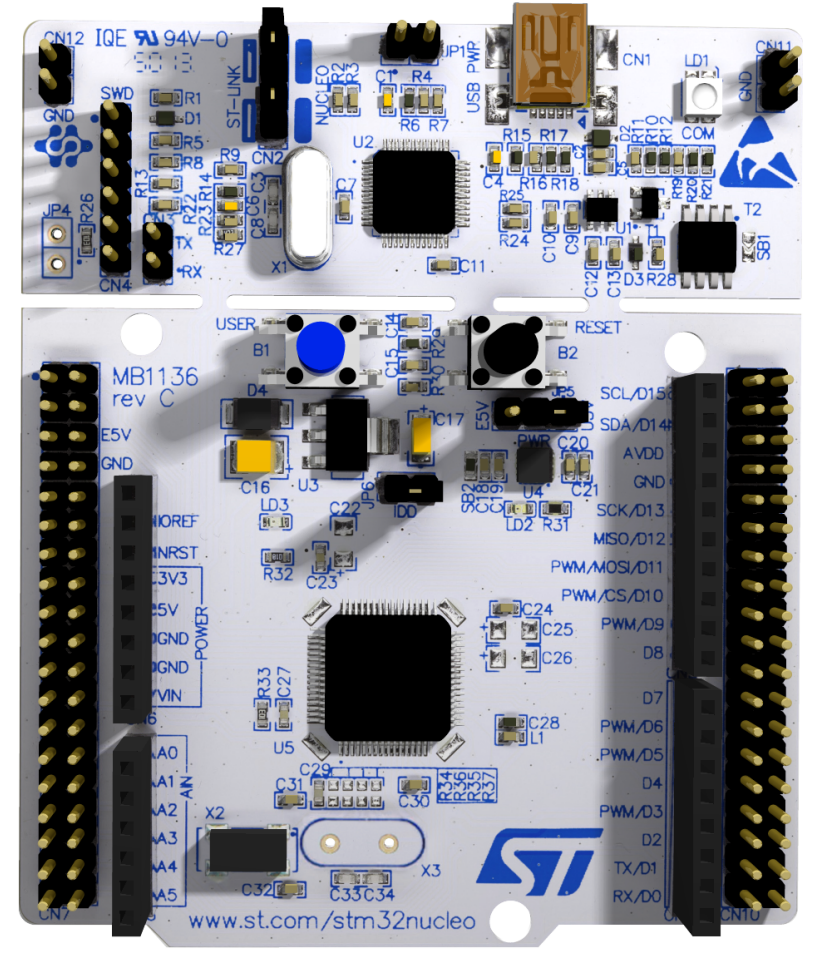
\includegraphics[width=6in, height=3.85in, keepaspectratio]{figures/nucleo64.png}
	\caption{STM32 Nucleo-64 Development Board \cite{nucleo64_manual}}\label{fig:nucleo64}
\end{figure}

\section{Interconnect PCB}
The interconnect PCB is a custom designed board with three goals: regulate voltage, route power, and connect peripherals to the development board. The PCB routes input battery power to two external buck regulators, producing 12 V and 7 V. The 7 V bus is further regulated to 5 V and 3.3 V logic rails using two AZ1085CD LDOs and then routed to the development board, sensors, etc. Most importantly, the interconnect board provides dedicated 2.0 mm JST connectors for all sensors, motor drivers, and the servo to simplify and robustify wiring across the robot. In addition, hand-crimped cables made with JST connectors and 28 gauge ribbon cable prevent rats nest wiring. A block diagram is shown in Figure \ref{fig:interconnect_block}. Due to uncertainty in the final robot design, extra hardware and circuits were added. Table \ref{tab:interconnect_features} lists the supported features. 

\begin{table}[h]
	\centering	\caption{Interconnect PCB -- Supported Features}
	\begin{tabular}{cl}
		\hline 
		Quantity & \multicolumn{1}{c}{Feature} \\ \hline 
		6 & VL53L0X laser rangefinder \\ \hline 
		1 & Adafruit 9-DOF IMU \\ \hline
		3 & Dual H-bridge motor driver \\ \hline
		2 & 5 V Standard servo \\ \hline
		2 & 8 sensor IR proximity array \\ \hline
		4 & Debug LEDs \\ \hline
		1 & Debug button \\ \hline
		1 & Reset button \\ \hline
	\end{tabular} 
	\label{tab:interconnect_features}
\end{table}

The system utilizes two 400 kHz I\textsuperscript{2}C buses to improve communication bandwidth with the numerous I\textsuperscript{2}C devices. Table \ref{tab:i2c_table} lists I\textsuperscript{2}C device addresses and bus allocation. The two buses are named I2C2 and I2C3 to maintain parity with the microcontroller's naming convention.

\begin{table}[h]
	\centering	\caption{Interconnect PCB -- I\textsuperscript{2}C Devices}
	\begin{tabular}{lcc}
		\hline 
		\multicolumn{1}{c}{I\textsuperscript{2}C Bus} & Device & Address (7-bit) \\ \hline 
		I2C2 & Rangefinder 4 & 0x52 \\ \hline 
		I2C2 & Rangefinder 5 & 0x53 \\ \hline 
		I2C2 & Rangefinder 6 & 0x54 \\ \hline 
		I2C2 & Adafruit 9-DOF IMU Gyroscope & 0x69 \\ \hline
		I2C2 & Adafruit 9-DOF IMU Accelerometer & 0x19\\ \hline		
		I2C2 & Adafruit 9-DOF IMU Magnetometer & 0x1E \\ \hline		
		I2C2 & GPIO Expander 3 & 0x3A \\ \hline				
		I2C3 & Rangefinder 4 & 0x52 \\ \hline 
		I2C3 & Rangefinder 5 & 0x53 \\ \hline 
		I2C3 & Rangefinder 6 & 0x54 \\ \hline 
		I2C3 & GPIO Expander 1 & 0x38 \\ \hline				
		I2C3 & GPIO Expander 2 & 0x39 \\ \hline				
	\end{tabular} 
	\label{tab:i2c_table}
\end{table}

The schematic capture and board layout were created in CadSoft EAGLE 7.4 due to its simplicity of use, popularity, and community support. The schematic can be found in Appendix \ref{appendix:schematic}, layout in Appendix \ref{appendix:layout}, and bill of materials in \ref{appendix:pcb_bom}. The board uses two  1 ounce copper layers for cost effectiveness. Two large headers underneath the board connect to the headers on the top of the microcontroller development board while the JST connectors are placed across the top of the PCB. 18-gauge wires soldered to large plated through-holes at the right edge of the board connect the external buck regulators. All components are placed on the top side of the board (except for the development board connectors) to make hand-soldering easier. The completed electronics assembly is shown in Figure \ref{fig:full_electronics}.

\begin{figure}[H]   % [h] means here
	\centering 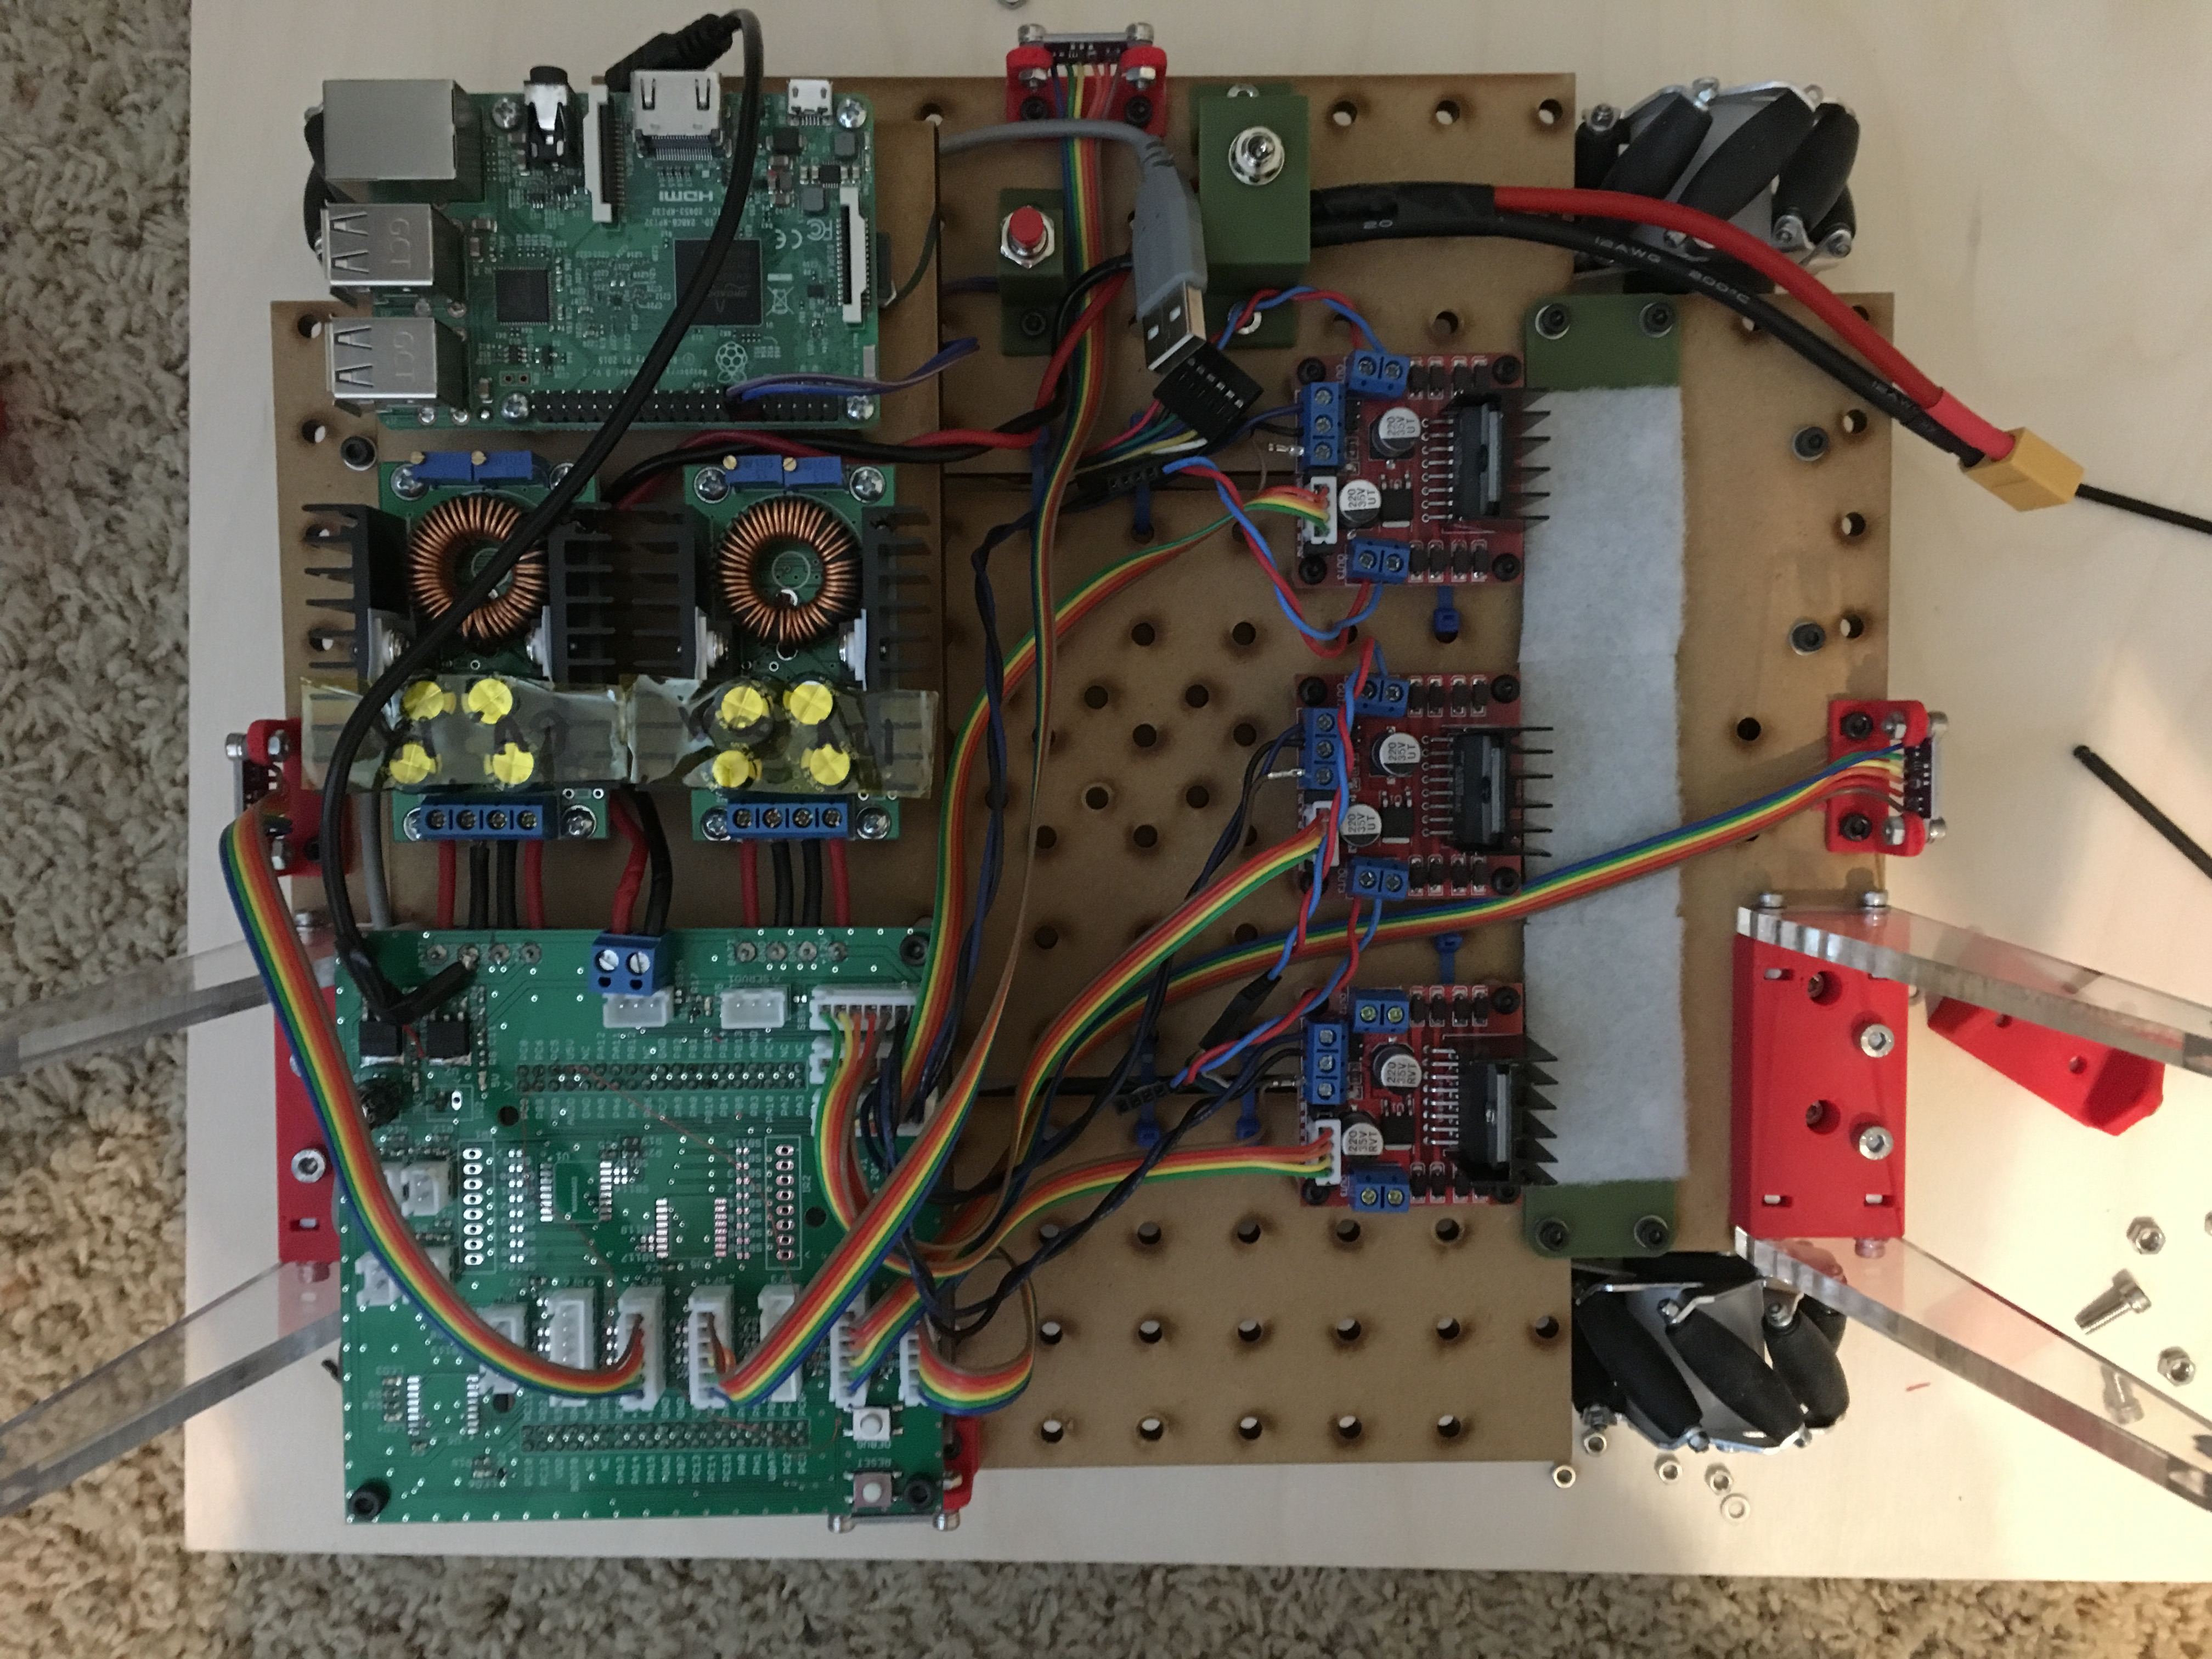
\includegraphics[width=6in, height=3.85in, keepaspectratio]{figures/full_electronics.jpg}
	\caption{Fully Assembled Electronics}\label{fig:full_electronics}
\end{figure}

